\chapter{Background and Literature review}%The Galician CTZ}
\label{ch:litrev}
\section{Regional Settings And Area Characteristics}

The general  bathymetry and coastal morphology of the west coast
of the Iberian Peninsula extends between latitudes 36\deg and
44\deg N (Fig~\ref{fig:largebathy}. It includes the typical
physiographic aspects of the continental shelf, the slope and the
rise.
\begin{figure}
 \begin{minipage}[b]{.35\textwidth}
 \includegraphics[scale=0.11]{bathy}
\end{minipage}
 \begin{minipage}[b]{.5\textwidth}
 \caption[Bathymetry of the Region]
 {Bathymetry and coastal morphology from GEBCO
 database showing the main features off the coast of
 Iberia from 44\deg N to 36\deg N and between 13\deg W and 8\deg W.
 Bathymetric contours at 200m and multiples of 1000m are shown.
 GB-Galician Bank, PC-Porto Canyon, AC-Aveiro Canyon, NC-Nazare
 Canyon, SC-Set\'{u}bal Canyon, VGS-Vasco de Gama Seamount,
 VS-Vigo Seamount, PS-Porto Seamount, GoB-Gorringe Bank.}
 \label{fig:largebathy}
 \end{minipage}
 \end{figure}
 The margin is cut in several places by submarine canyons which
generally define boundaries between regions with relatively
similar bathymetry conditions. North of the Nazar\'{e} canyon the
shelf is wide and very flat, with the exception of the Porto and
Aveiro canyons, as far as Cape Finisterre. Offshore of the shelf
edge, indicated by the isobath of 200m, the bottom topography is
quite complex. Between latitudes 43.5\deg and 41\deg N the
bathymetry is characterised by a deep meridional valley with a
maximum depth of 2800m separating the continental slope from the
Galicia Bank (minimum depth of 560m) to its west. The shoreline
extends almost meridionally up to about 42\deg N and then the
coast presents strong indentations (the 'Rias Bajas') as far as
Cape Finisterre. Further south at 41\deg N latitude, the Vigo,
Porto and Vasco de Gama seamounts are found. Between Nazar\'{e}
and the Lisbon region, the shelf is more irregular and is
dominated by a well pronounced zonal ridge. South of the
Set\'{u}bal canyon, the shelf is fairly flat as far as Cape Sines,
beyond which it becomes very steep until Cape S\~{a}o Vicente,
practically without a shelf break. The coastline is again
orientated very nearly in the meridional direction. At the
latitude of Cape S\~{a}o Vicente a large ridge extends offshore.
Freshwater input to the Galician shelf from the Rias (four in the
west coast and 3 in the north coast) and the Minho river is small
during summer (204\tra from mid May to mid October)
\citep{Huthnance02} but increases in winter.


\subsection{General circulation in the North Atlantic} The general
circulation in the North Atlantic (Fig.~\ref{fig:gencirc}) is
characterised by the presence of two large wind-driven gyres: the
cyclonic subpolar gyre and the anticyclonic subtropical gyre. The
subtropical gyre has its Northwest boundary defined by the Gulf
Stream (GS) which is responsible for the recirculation of the gyre
\citep{Dietrich75}. Southeast of the Grand Banks the GS separates
into two branches: the North Atlantic current, flowing to the
Northeast and feeding the subpolar gyre \citep{Clarke80,Sy88}; and
the Azores Current (AC), which crosses the North Atlantic to the
East coast between 35\deg N and 30\deg N, the exact position being
subjected to seasonal displacements \citep{Tokmakian93}.
\citet{Stramma84}, on the basis of geostrophic calculations on the
historical archive of hydrographic data, found that the eastward
flowing AC separates into three branches as it turns southward on
approaching the eastern boundary. Two branches separate west of
Madeira to make up an interior southward recirculation of the
subtropical gyre while the third passes north and around Madeira
to feed into the Canary Current.
\begin{figure}
  \centering
  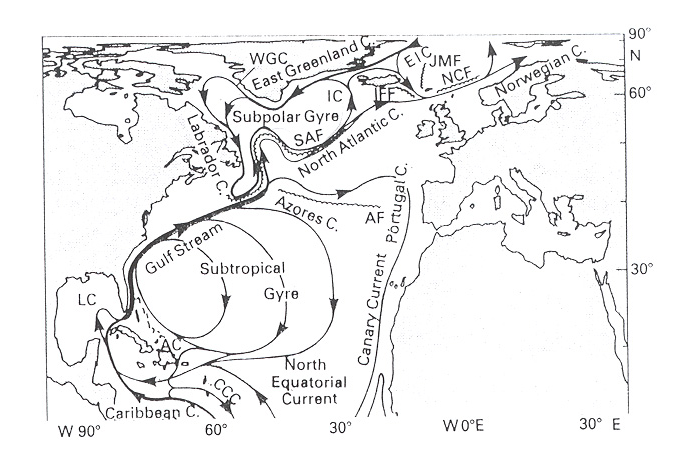
\includegraphics[height=6.5cm,width=10cm]{fig2}
  \caption{General surface circulation of the North Atlantic
  (after {\it Tomczak and Godfrey,} 1994). Abbreviations are used for
  the West Greenland Current (WGC), Irminger Current(IC), East
  Iceland Current(EIC), Loop (LC) and Antilles Currents(AC) and
  the Caribbean Countercurrent (CCC). Other Abbreviations refer to
  fronts:  Jan Mayen Front (JMF), Norwegian Current Front (NCF),
  Iceland-Faroe Front (IFF), Subartic Front (SAF) and Azores Front
  (AF).}\label{fig:gencirc}
\end{figure}

A consistent weak eastward flow of Eastern North Atlantic Central
Waters (\enaw) appears to exist off the Iberian Coast from north
of the Azores Current at depths of 200-300m corresponding to
densities lower than 27.25
\citep{Saunders82,Pollard85,Arhan94,Maze97} consistent with a
poleward shoaling of isopycnals \citep{Barton02}. Part of that
flow is later diverted off the south coast of Portugal towards the
gulf of Cadiz \citep{Maze97}. This zonal flow is associated with a
northward flow and downward entrainment with  40\% of the \enaw
entering the Mediterranean Intermediate Water (MIW) layer
\citep{Maze97} although seasonal variability can be expected in
its dynamics \citep{Saunders82,Arhan94}.

The Mediterranean outflow at the strait of Gibraltar forms MIW and
travels along the Algarve continental slope to spread out
ultimately into the Atlantic at depths between 600 and 1500m. The
MIW is evident as two maxima of temperature and salinity cores
\citep{Daniault94} and its flow is characterized by a westward
advection (mainly raised by mesoscale features as shedding eddies,
MEDDIES \citep{Kase89,Haynes90}) and turbulent diffusion of MIW
together with a well defined northward jet along the Iberian shelf
break and slope (Fig~\ref{fig:circmw}) \citep{Meincke75,Arhan94}.
The northward flow of MIW enters the Iberian slope by the Tagus
Bank between Cape S\~ao Vicente and the Gorringe Bank
\citep{Zenk90} and was named the Portugal Slope Undercurrent (PSU)
by \citet{Ambar94}. Part of the flow separates there from the
slope and flows back southwestward to the west of the Gorringe
Bank (Fig.~\ref{fig:circmw}) while the rest of the flow proceeds
northward in the form of a Slope Undercurrent \citep{Daniault94}
with a characteristic transport of 7.6 $10^6$ \tra \citep{Maze97}.
The MIW slope current divides later into two branches between
41\deg N and 42\deg N, a western branch flowing to the west of the
Galician bank and a coastal branch following the shelf break in
response to the  steering effect of bottom topography.  A further
effect of the bottom topography-flow interaction of the PSU is the
existence of a bottom boundary Ekman layer enhancing downslope
Ekman transport.

In the same region the Central Waters flow strongly resembles that
of the MIW, suggesting a vertical coupling of both water masses.
\begin{figure}
  \centering
  \includegraphics[height=11cm,width=9cm]{fig3}
  \caption{Schematic circulation of MW in May 1989 in the Iberian
  coast. Black dots represent CTD stations. Reported numbers are volume
  transports in $10^6$ \tra [from {\it Maz\'e et al.,} 1997].}
  \label{fig:circmw}
\end{figure}
\subsection{Weather Regime} Upwelling occurs all along the East
coast of the central North Atlantic from the northern tip of the
Iberian peninsula to south of Dakar at almost 10\deg N, as a
result of the characteristics of the wind. During the summer
months, when the Azores high-pressure cell is located in the
central Atlantic and the Greenland low has diminished in
intensity, the resulting pressure gradient forces the air to flow
southward along the coast of Iberia inducing upwelling and
associated southward circulation. In contrast, in winter the
Azores high-pressure cell is located further south, off the
northwestern African coast, and a deep low is located off the
southeastern coast of Greenland. The pressure gradient between the
two pressure systems results in an onshore wind with a component
of wind stress northward off Iberia.

\citet{Blanton87} showed that there are large interannual
variations in upwelling in response to the large-scale meteorology
variations in the North Atlantic. The continuously varying
strength and position of the Azores High and the Greenland Low
lead to variations in the strength and direction of upwelling
favourable winds at these latitudes.

\subsection{Coastal circulation} The general structure of the
Portugal Current System off the west Iberian coast is formed by
the following basic components \citep{Fiuza96b}:
\begin{enumerate}
  \item  a large scale southward surface flow in the open ocean,
  seaward of the continental margin related to the N. Atlantic
  subtropical gyre, the Portugal Current,
  \item an equatorward surface flow over the slope, in the
  vicinity of the shelfbreak during the upwelling season
  (June-July until late September), the Portugal Coastal Current,
  \item a poleward surface flow along the upper slope from
mid-autumn until late spring, the Portugal Coastal Countercurrent,
  \item the semi-permanent poleward Portugal Slope Undercurrent.
\end{enumerate}
Bearing in mind that none of the above currents are restricted to
the Portuguese margin they would be better named the Iberian
currents.
\subsubsection{Winter regime}
\begin{figure}
  \centering
  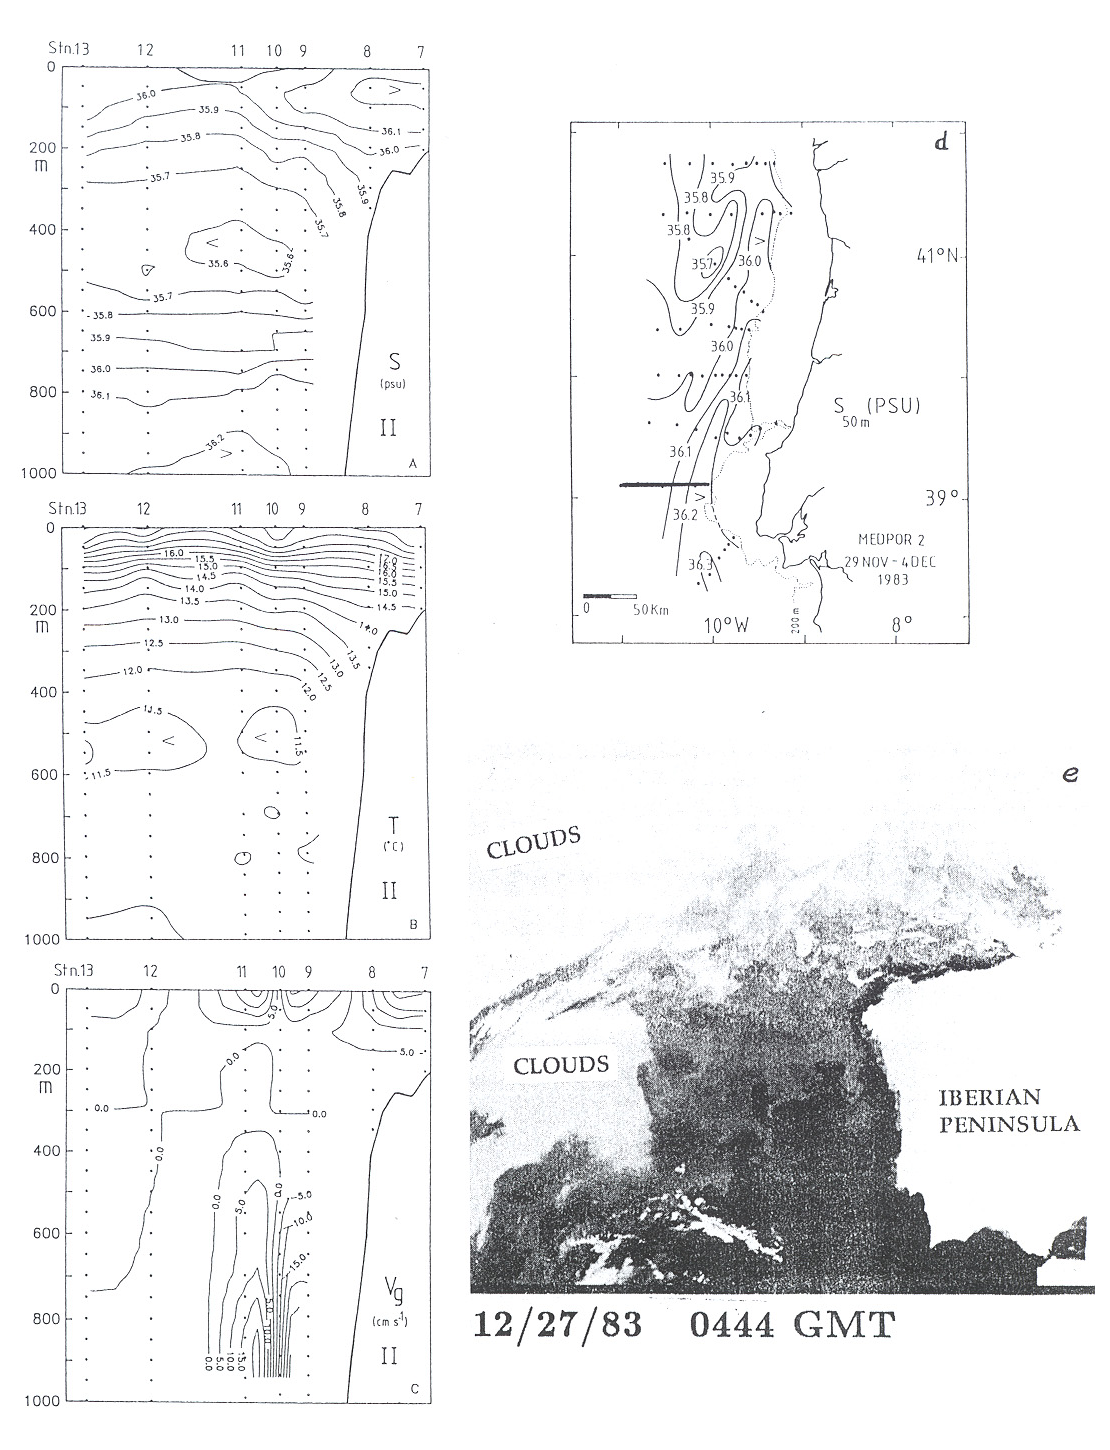
\includegraphics[width=16cm]{fig4new}
  \caption{Different signatures of the PCC from winter 1983.
  Vertical distribution of (a) salinity, (b) temperature, and (c)
  meridional component of geostrophic velocity relative to 300
  dbar along section II (thick line in d). Salinity distribution
  at 50m (d) showing the PCC (saline intrusion) along the slope.
  Thermal infrared picture (e) from the NOAA 7 satellite where
  darker tones corresponds to warmer temperatures [from {\it Frouin et
  al.,} 1990].}\label{fig:poleward}
\end{figure}
The meteorological conditions offshore from the Iberian Peninsula,
governed by the meridional displacements of the Azores High as
mentioned before, show distinct winter and summer regimes.  In
winter, the weakening and southward migration of the anticyclone
places the north of the region under the influence of
southwesterly winds. The upper layer circulation in this season is
characterised by the presence of a narrow northward slope current
which settles in November and disappears around May
\citep{Frouin90,Haynes90,Pingree92}. This structure
(Fig.~\ref{fig:poleward}) appears as a warm and saline intrusion
(temperature 1-3\deg C and salinity 0.2-0.3psu higher than
surrounding values), trapped within about 50km of the shelf break,
about 200-600m deep. It flows along the slope with characteristic
velocities of 0.2-0.3\vel, and extends more than 1500km and with
transport increasing in the flow direction
\citep{Frouin90,Haynes90}. Drifter experiments
(Fig.~\ref{fig:morenadrifters}) have revealed a meandering surface
flow with eddies of different scales superimposed on the poleward
mean flow \citep{Haynes91,Sena96}. This Portugal Coastal
Countercurrent (PCC),\citep{Fiuza97}, flows along a semi-permanent
front separating the fresher shelf waters influenced by the winter
river runoff from rivers of northern Portugal particularly from
the Douro, from the open ocean \citep{Hamann96}. That convoluted
front was observed to contribute to the shelf-ocean exchange via
mesoscale cyclonic eddies (10-20km in diameter) which are shed
into the open ocean from the Countercurrent
\citep{Fiuza96b,Perez01}. Other active exchange processes are
mixing and entrainment into the poleward Countercurrent of shelf
waters which are advected alongshore for hundred of kilometres
before dispersing into the open ocean with an estimated residence
time on the shelf of 1-2 months\citep{Fiuza96b}. Those fronts are
common features of the shelf breaks as a result of buoyancy inputs
and their ``anchorage" at the shelf break is a response to
potential-vorticity conservation and geostrophy \citep{Condie93}.
As mentioned above, the slope current extends downwards including
the MIW to a depth of 1500m and more, as reported by
\citet{Huthnance02} at various moorings along the Iberian Atlantic
coast outside the shelf break.
\begin{figure}
  \centering
  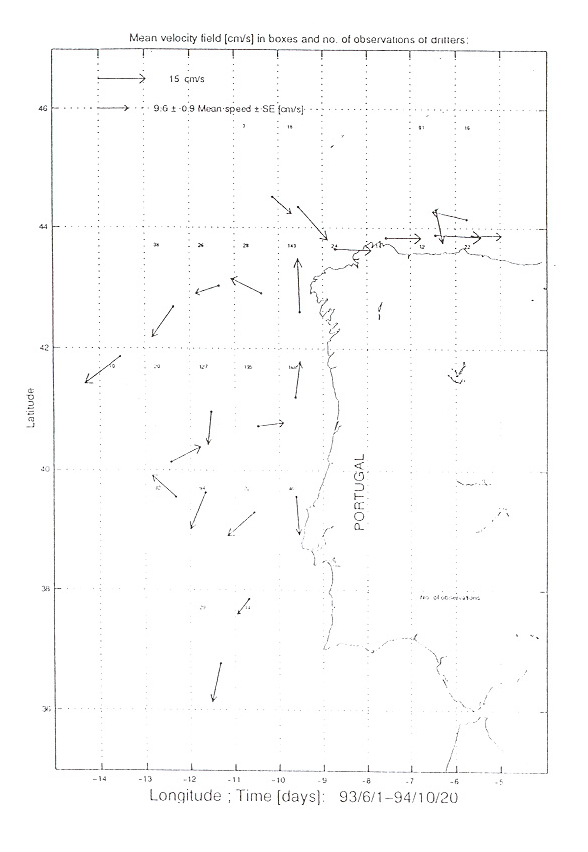
\includegraphics[height=9cm]{fig5anew}
    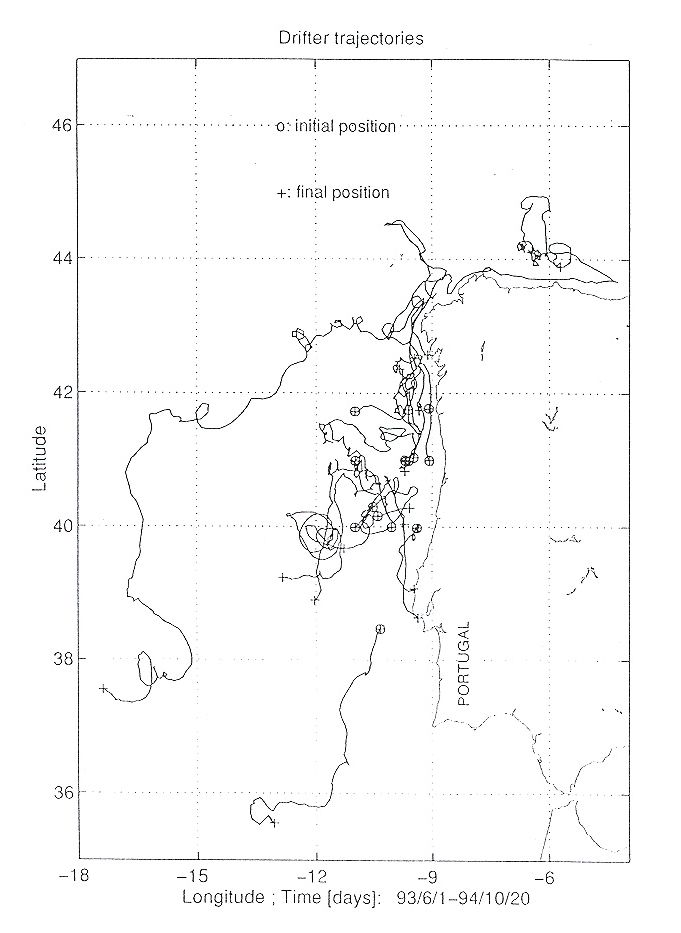
\includegraphics[height=9cm]{fig5bnew}
  \caption{Mixed layer drifter tracks (right) and derived surface
  velocities (left) for 16 drifters used in the MORENA project
  during June 1993-October 1994. 11 drifters were released during
  November 1993 and their trajectories correspond to the period
  November 1993-May 1994 [{\it Sena,} 1996].}\label{fig:morenadrifters}
\end{figure}

\citet{Pollard85} described a meridional density gradient in the
upper 200-300m associated with the poleward cooling of the sea
surface which can force a poleward current that becomes
intensified over the slope and which increases along the flow
\citep{Huthnance84}. The winter wind circulation could also
generate a poleward slope current and the two mechanism were found
to actively drive the PCC \citep{Frouin90}.

Large and persistent anticyclonic warm slope-water eddies
(SWODDIES) have been associated with the PSU in winter if the warm
flow is strong \citep{Pingree94} in relation with the instability
of the slope current in the Bay of Biscay
(Fig.~\ref{fig:swoddies}) although no consistent seasonal
variability has been established. They have characteristic radii
of 50-60km, a signature discernible in the upper 1500m, and a
lifetime of about a year. \citet{Pingree93} also identified eddies
shed from the slope at Cape St. Vincent, Setubal canyon and Lisbon
canyon in respond to the complex topography
(Fig.~\ref{fig:swoddies}b and c) and the persistence of a
topographic eddy is suspected over the Galician Bank
\citep{Hill98}.

There has been reported evidence of poleward flow south of 35\deg
N \citep[i.e. off NW Africa][]{Barton90,Mittelstaed91} which shows
seasonal persistence, although its connection with the PCC is not
yet established.
\begin{figure}
  \centering
  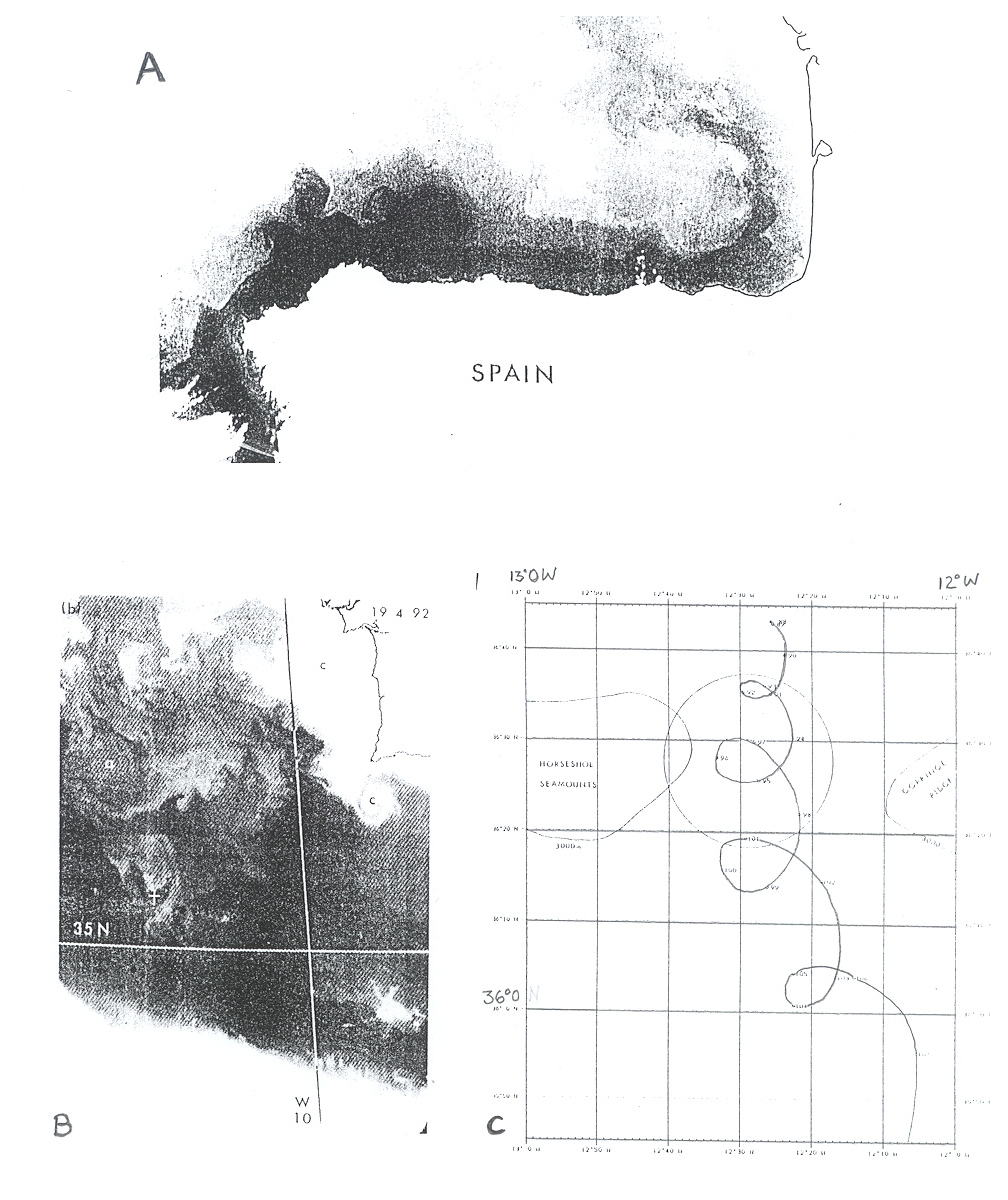
\includegraphics[height=14cm]{fig6new}
  \caption{Eddy signatures along the Iberian coast. (a)  Infrared
  image (NOAA 10, 28 Dec. 1989) showing warm surface water flowing
  along the west and northern Spanish slopes and swoddy formation.
  (b) Infrared image (NOAA 12, May 5, 1992) showing the
  development of a cyclonic eddy off Cape St. Vincent (labelled
  c). (c) Track of buoy 3906 (drogued at 800m) with daily
  positions marked, showing typical 4-day period and southward
  translation (~5km/d). A circle of 35km is shown to indicate the
  scale of the eddy core. ((a) from {\it Pingree and LeCann} 1990, (b,c)
  from {\it Pingree and LeCann} 1993).}\label{fig:swoddies}
\end{figure}
\subsubsection{Summer regime} In the North Atlantic the summer
Trade winds have a strong alongshore component which drives
upwelling off Iberia from May to October as described in the early
works of \citet{Wooster76} and \citet{Fiuza82b}. A more detailed
study of the wind regime in the coasts of the Iberian Peninsula
was made by \citet{Bakun91} who calculated wind stress and curl of
wind stress on a 1x1\deg  grid from historical merchant ship
records. Their results showed that the near shore region from
Iberia to 15\deg N is characterised generally by cyclonic
wind-stress curl (Positive) during the upwelling season, which
causes in turn a divergence and consequent Ekman pumping enhancing
the coastal upwelling. However, local wind patterns near the coast
may be significantly affected by orographic influences due to the
presence of capes and Rias locally enhancing upwelling
\citep{Mcclain86}.

The upwelling favourable winds during the summer have a marked
oscillatory pattern from March till October as revealed by
harmonic analysis of 9 years of daily averaged upwelling indices
deduced from geostrophic winds estimated for a cell centred at
43\deg N 11\deg W, 150km off Cape Finisterre \citep{Nogueira97}.
The wind displays a quasi-periodic component of T=15$\pm$5 days
during the upwelling season. This time structuring is imposed on
the shelf ecosystem and is in part responsible for the high
productivity of the area. Further south, in the Portuguese
Atlantic coast, periods were found to be of 6-7 days
\citep{Sousa86}. \citet{Nogueira97} also concluded that the
downwelling season has a less regular pattern, with the dominant
mode of variation being T$\sim 30\pm$20 days.
\begin{figure}
  \centering
  \includegraphics[height=6cm,angle=-90]{fig7anew}
  \includegraphics[height=6cm,angle=-90]{fig7bnew}
  \includegraphics[height=12cm]{fig7c}
    \caption{(a) Location of stations sampled in August September
  1981. (b) Section showing the meridional component of
  geostrophic velocity (computed relative to 300 dbar and
  expressed in \velc ); negative values represent southward flow
  [{\it Fiuza }1983]. (c)Temperature distribution at 50dbar in September
  1994 showing the anchorage of the upwelling front to the shelf
  break [{\it Fiuza }1996].}
  \label{fig:summerupw}
\end{figure}

 Continental shelf and slope waters off the western and southern
Iberian Peninsula are dominated during the summer months by strong
coastal upwelling. The associated baroclinic equatorward jet
(Fig.~\ref{fig:summerupw}), the Portugal Coastal Current (PCoC)
\citep{Ambar94}, attains velocities of 15-20\velc
\citep{Fiuza84,Mcclain86}. A strong temperature front, separating
the cold recently upwelled water from the offshore oceanic water
(Fig.~\ref{fig:summerupw}), develops in close relation to the
bathymetry of the continental shelf and slope and to the coastal
morphology \citep{Fiuza83}. The time response of the system to
local wind forcing was estimated by \citet{Sousa86} to be less
than 24hrs in the Portuguese coast, as expected from such a
dynamic system, although \citet{Mcclain86} give values of 3 days
for the Galician coast. The time evolution of the system includes
further distortion of the front and development of meanders,
eddies and filaments following a seasonal pattern
\citep{Haynes93}.

During the upwelling period, the wind forcing is opposite to the
poleward density gradient but the PCoC equatorward geostrophic jet
is enough to counter the poleward slope current at and near the
surface so that southward flow is established. However, below
100-200m the flow is still poleward \citep{Haynes90,Huthnance02}.
Spectral analysis of long-term moored current-meters have shown
the presence of signals in the period range of 40-70hrs, which
match the characteristics of the second mode of continental shelf
waves compatible with the local stratification and bottom
topography \citep{Fiuza96}. This waves could play a significant
role in accommodating the eastward flow of ENAW
\citep{Huthnance95} and in driving part of the poleward
undercurrent as suggested in the Californian upwelling system
\citep[e.g.][]{Wang97}. Their relevance in the Iberian system is
yet to be established.

\subsubsection{Patterns of mesoscale variability}
Early in the eighties, \citet{Fiuza83} suggested the strong
3-dimensionality of the Iberian Upwelling system identifying an
upwelling front strongly deformed by meanders, mesoscale eddies
and filaments (Fig.~\ref{fig:litomexfil}), cold tongues of
recently upwelled waters extending offshore some hundreds of km.
Capes such as Cape St. Vincent \citep{Sousa86,Relvas99}, or Cape
Finisterre \citep{Blanton84} are also involved in the promotion of
localized or intensified coastal upwelling introducing an
important component of spatial variability into the system.
\begin{figure}
  \centering
  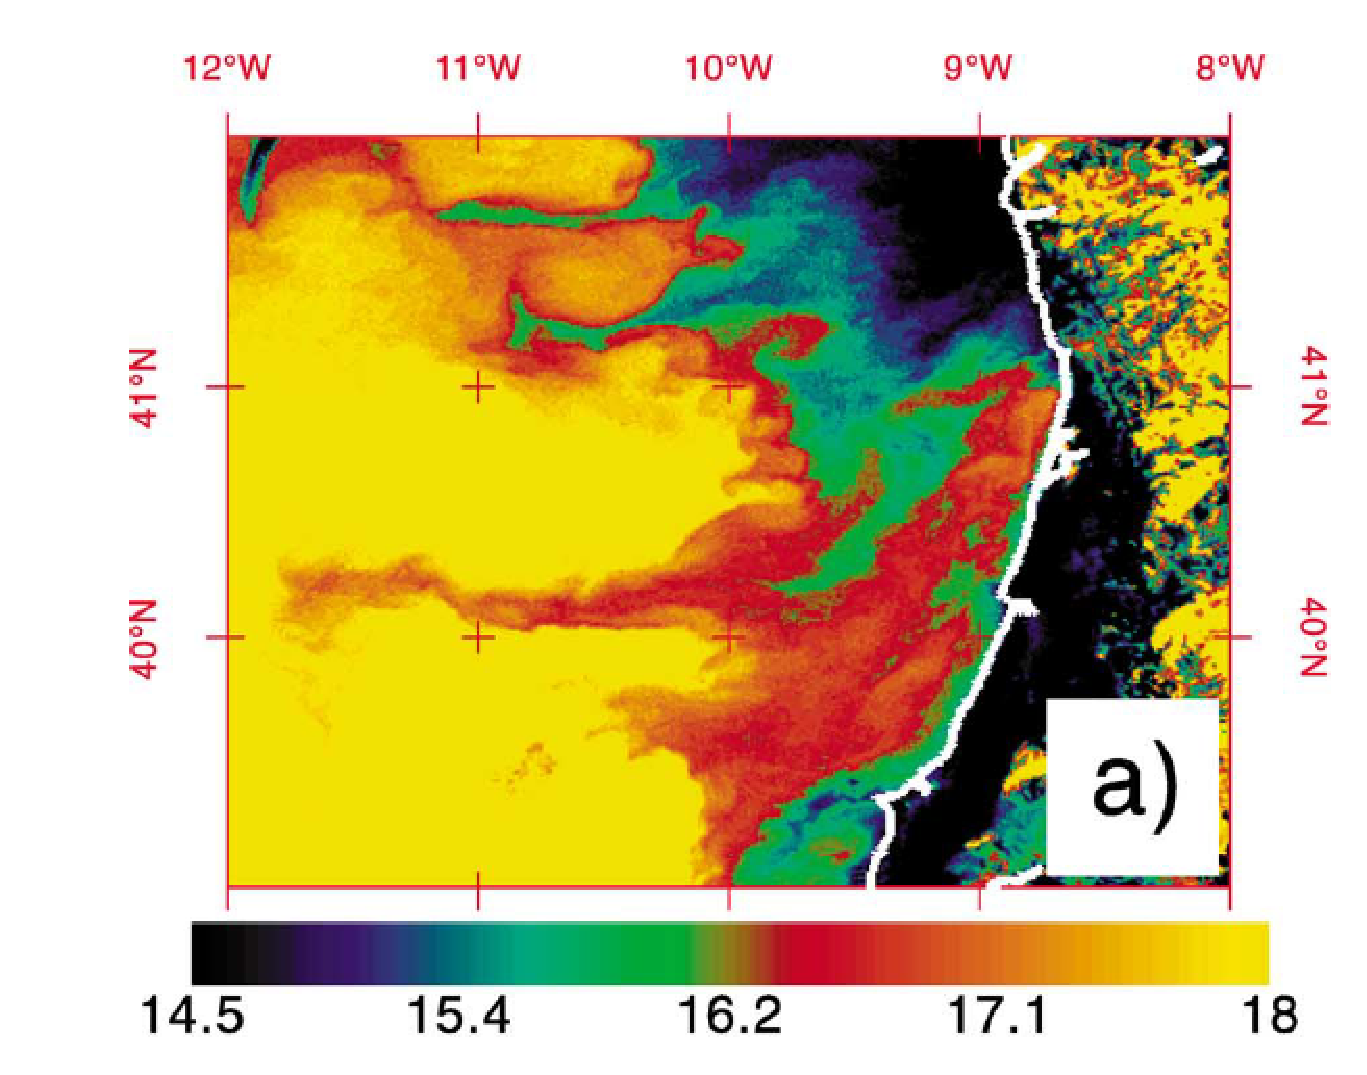
\includegraphics[height=10cm]{filaments}
  \caption{AVHRR Channel 4 brightness temperatures of the Western
  Iberian coast. (a) NOAA-14 in 24/08/98 at 03:58 UTM.
 The HRPT data were received at the Dundee
Satellite Receiving Station and processed at IPIMAR [{\it Peliz et
al., }2002] }
  \label{fig:litomexfil}
\end{figure}

The large mesoscale features of the region, in particular the
filaments, follow a strong seasonal fluctuation similar to the
California Upwelling System, in strong relation to the seasonal
wind pattern. At the beginning of the upwelling season, May-June,
a narrow band of colder water of quite uniform width develops
along the coast, often consisting of many narrow ``fingers'' of
cool water extending 20-30km offshore \citep{Haynes93}. Those
features have been successfully modelled in a 1\onehalf \, layer
model by \citet{Roed96} for the Iberian region including realistic
topography and coastline geometry. Linear stability analysis has
also suggested that front waves of wavelengths about 20km appear
first \citep{Barth94} in response to frontal instability
\citep[e.g.][]{Washburn88,McCreary91}] which feeds from potential
energy stored in the lateral density gradient.

\begin{figure}
  \centering
  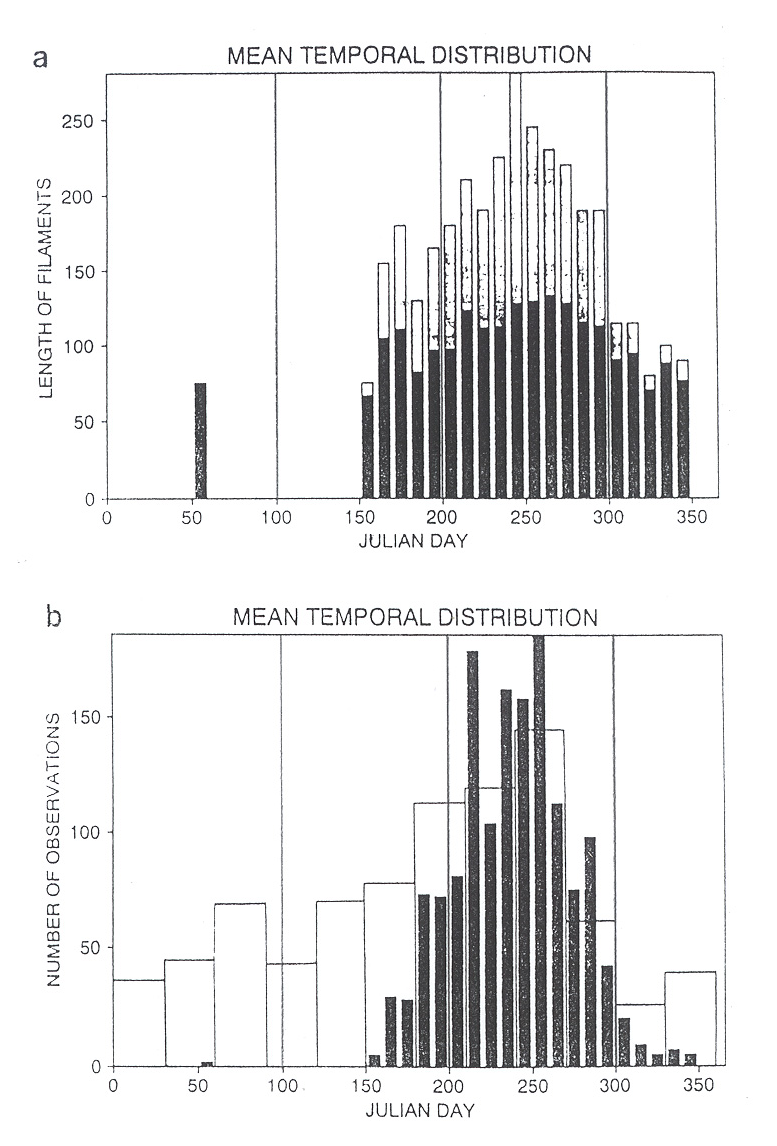
\includegraphics[height=16cm]{fig9new}
  \caption{(a) Temporal evolution of the mean length (solid bars)
  and greatest observed lengths (grey bars) of filaments from the
  brightness temperature scene archive (1982-1990). (b) Temporal
  evolution of the number of observed filaments per 10 day
  interval (solid bars). Open bars indicate the number of images
  available for 30-day periods [{\it Haynes et al., }1993].}
  \label{fig:filstats}
\end{figure}
The narrow band might temporarily disappear after relaxation or
poleward wind events and is not until July or August that the
fingers merge in preferred locations to form filament structures.
Statistical analysis from \citet{Haynes93} spanning over 9 years
(1982-1990) showed filaments reached a mean length of 80km (30km
seaward of the upwelling coastal band) in July and then continued
growing until reaching a maximum mean length of 130km in late
September (Fig.~\ref{fig:filstats}). Similar growth rates were
found for the largest filaments which can reach over 250km in late
September. Filaments seem to weaken towards the end of October and
to disappear on a time scale of the order of a week once upwelling
stops \citep{Haynes93}. Similar seasonal increase in the strength
of mesoscale meanders, filaments  and eddies was observed for the
Californian System during one year GEOSAT altimeter data by
\citet{Flament89}. The expected lifetime of the filaments ranges
from 1 to 3 months \citep{Haynes93,Sousa95}.

\citet{Strub91} suggested three possible mechanisms for filament
formation, namely ``squirts'', meandering jet and pre-existent
eddy field. Only the  first two were identified as possible
generating processes in the Iberian System \citep{Haynes93}.
``Squirts'' respond to nearshore convergences while the meandering
jet has been identified as a consequence of baroclinic instability
and both are affected by the coastline and bathymetry as suggested
by \citet{Sousa92} and \citet{Haynes93} for the Iberian filaments.
The pre-existent eddy field implies that eddy pairs interact to
drag cold water seaward but the deterministic nature of the
filaments means that a truly random interaction of oceanic eddies
with the coastal transition zone is not possible.
%\begin{figure}
%  \centering
%  \includegraphics[height=18cm,width=14cm]{blank}
%  \caption{Meridional temperature profiles along part of the
%  Iberian coast ( 42.5\deg N-40\deg N, 10\deg W) during the upwelling season
%  of 1982 together with the bathymetry section of the same line at
%  50km from the coast ({\it Mendes de Sousa} 1995).}
%  \label{fig:filridges}
%\end{figure}

\citet{Haynes93} identified 5 major filaments in the Iberian coast
which recur every year in the same position. They are associated
with topographic features of the region, mainly capes such as Cape
Finisterre and Cape Ortegal in the Galician coast of Iberia and
Cape Roca, Cape Sines and Cape S\~ao Vicente in the Portuguese
coast. Their results were later confirmed by \citet{Sousa95} in a
similar analysis of 11 years of AVHRR data (1979-1989) in which
filaments were consistently associated with submarine ridges.
Laboratory experiments in a rotating tank \citep{Narimousa89} have
successfully reproduced a meandering upwelling yet and filaments
in the presence of ridges owing to the topographic effect and
potential vorticity conservation. Modelling work done by
\citet{Roed96} also reproduced the observed distribution of the
Iberian filaments and their time persistence. Energy consideration
within the model identified frontal instability as the baroclinic
instability responsible for the generation and growth of eddies
and filaments, while potential vorticity considerations suggested
that coastline and topography irregularities provide sufficient
background perturbation for the frontal instability mechanism.
\begin{figure}
  \centering
  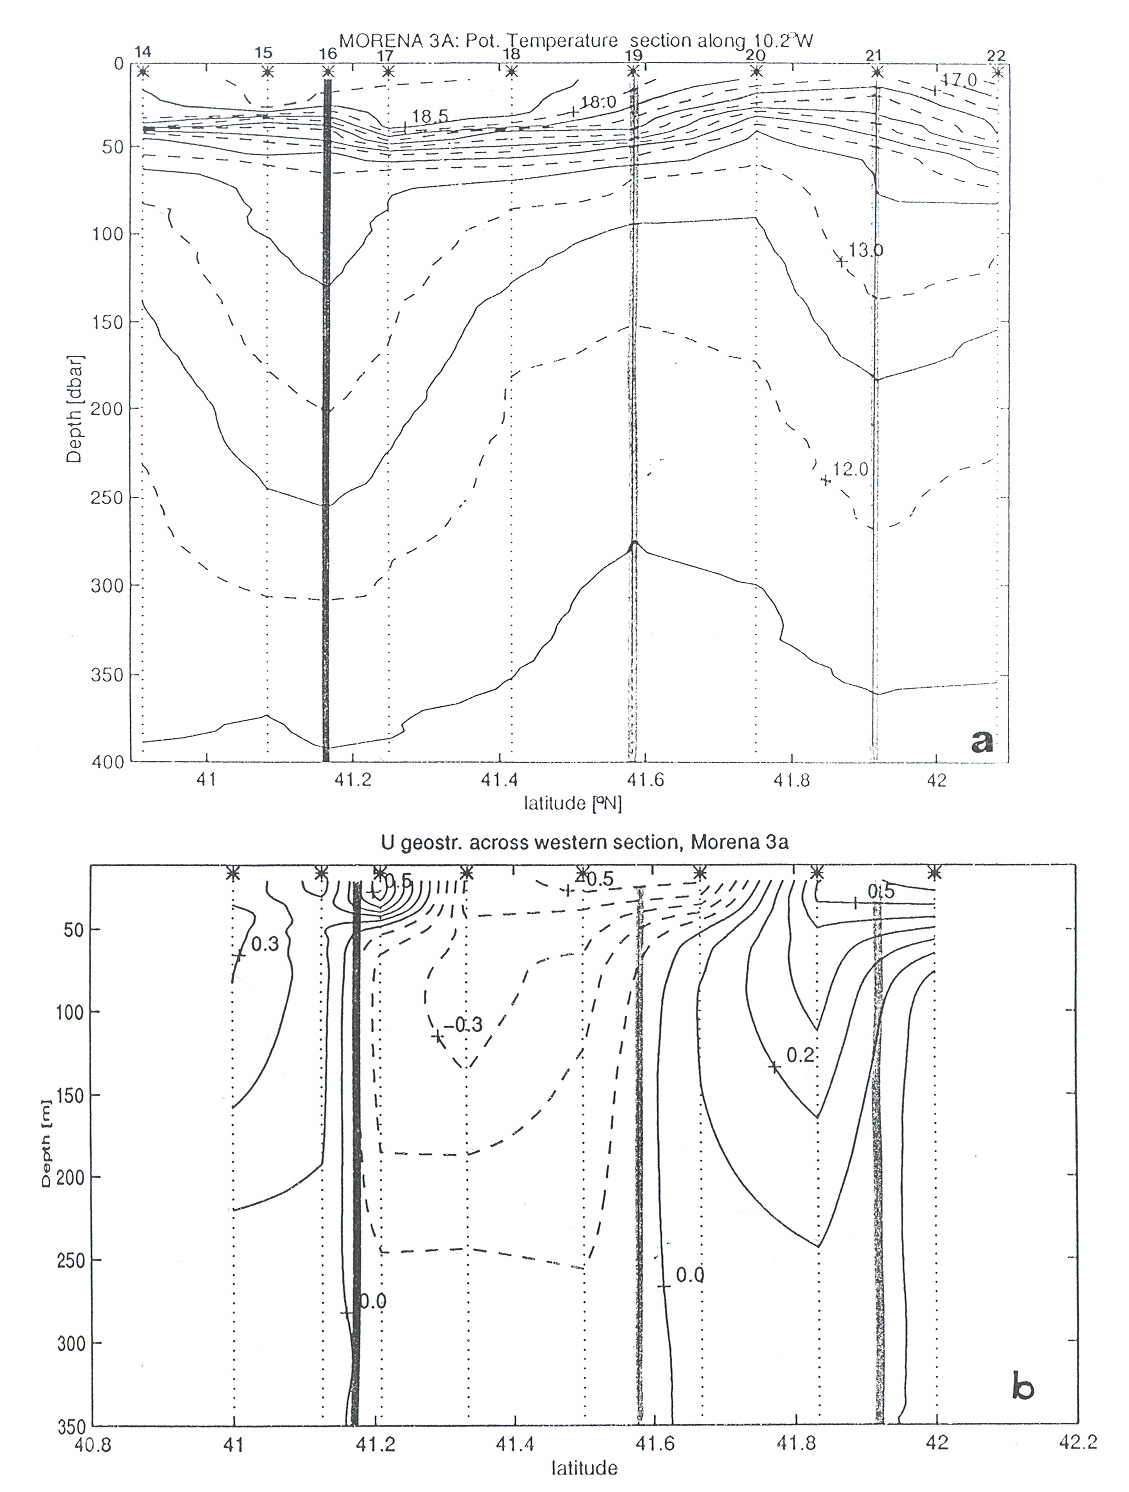
\includegraphics[height=16cm]{filamentsectionnew}
  \caption{(a) Meridional temperature section along 10.2 W carried
  out in the 6-7 August 1994 and (b) geostrophic velocity section
  along the same line calculated relative to 350dbar. Positive
  values indicate offshore velocities [{\it Fi\'uza }1996].}
  \label{fig:morenafil}
\end{figure}

Few in situ surveys have been carried out to determine the 3-d
structure of filaments,  the recent MORENA project being one of
the best examples \citep{Fiuza96b}. Hydrography and ADCP surveys
showed filaments extended 100-200km offshore. They were 30-50km
wide and penetrated to 250m deep  near their shelf-edge ``root'',
but diminished offshore  to 20-30km in width and 50m in depth. The
classical view of strong offshore baroclinic flow was supported by
the geostrophic velocities calculated from the hydrographic data
which displayed a surface core velocity of 0.5\vel decreasing to
about 0.05\vel\, at depths of 150-200m (Fig.~\ref{fig:morenafil}).
Some irreversible mixing of filament and ocean waters is expected
and filaments would play an important role in the exchange between
the shelf and ocean \citep{Huthnance95}.

Dynamic features of the upwelling system off the Western Iberian
coast, like the 'event' scale variability, the existence of a
frontal alongshore jet, and the omnipresent poleward slope
undercurrent have parallels in all the major upwelling regions
\citep{Barton98}. A summary of the main characteristic of the
Iberian upwelling can be seen in Table~\ref{tb:lit_summ}.
{\linespread{1}
\begin{table}[h]
  \centering
\begin{small}  \begin{tabularx}{400pt}{XXXXX}
  \textbf{Principal climatic influence} &\textbf{Principal Oceanic influence}  &\textbf{Topography}&\textbf{Freshwater
  influence}&\textbf{Winds}\\
  Azores High &Portugal Current&Narrow shelf&Small, Spanish Rias in the north&NE trades (summer) \\
  \hline
  \textbf{Tides}&\textbf{Poleward flow}&\textbf{Equatorward flow}&\textbf{Upwelling}&\textbf{Filaments}\\
  Internal tide generations, solitons&Along shelf edge, turn 90\deg to flow along North Spanish slope& Portugal Coastal Current&
  37\deg-43\deg N &130km mean, 270km maximum, 5 main sites\\
  \hline
  \textbf{Fronts}&\textbf{Eddies}&\textbf{Quasi-permanent eddies}&\textbf{Coastal Trapped Waves}&\textbf{Short-term variability}\\
  Upwelling fronts&Generated off Cape St Vincent&Over offshore banks?&Not known&Not known\\
  \textbf{Seasonal variability}&\textbf{Interannual variability}&\textbf{Special
  features}&&\\
  Upwelling in summer, Poleward flow in winter&Not reported&Divided from NW Africa eastern boundary by Strait of Gibraltar&&\\
  \hline \hline
  \end{tabularx}
   \end{small}
  \caption{Summary of Phenomena and Processes in the
  Iberian Eastern boundary.}\label{tb:lit_summ}
\end{table}
}
\subsection{Water-Masses in the Iberian coast }
The NW Iberian upwelling region is the least productive  of the
oceanic eastern boundaries \citep{Castro00}. Pacific and Indian
oceans present considerably higher nutrients and lower oxygen
levels than the Atlantic ocean \citep{Levitus93}. The Galician
coast is situated in the region of the ventilated thermocline
where \enaw forms \citep{Rios92}, and consequently, \enaw upwelled
along the Galician coast exhibits low nutrient enrichment by
oceanic ageing compared to \enaw that upwells off the African
coast \citep{Castro00}.

Different water masses can be identified off the Iberian Atlantic
coast where the water column can be divided into upper (first
100-200m), intermediate (to a depth of 1300) and deep (from 1300m
to the bottom) layers.
\begin{figure}
  \centering
  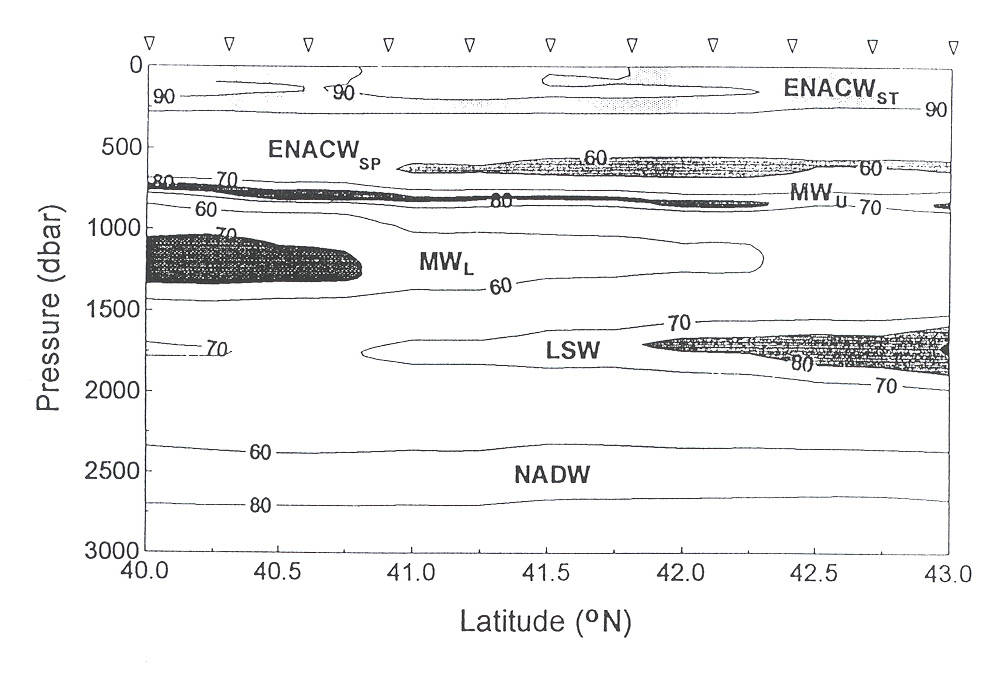
\includegraphics[width=13cm]{watermassnew}
  \caption{Percentages of the different water masses as indicated
  by their abbreviated designations (st and sp meaning subtropical
  and subpolar respectively), calculated using $\theta$/S mixing
  triangles along a meridional section at 10\deg W. The positions of
  the CTD stations collected during May 1993 are indicated by
  small triangles along the top of the figure [{\it Fi\'uza et
  al.,} 1997].}
  \label{fig:ctdmixing}
\end{figure}

The upper layer during winter months corresponds to a mixed layer
produced by wind stress mixing, of surface fresh water from
precipitation and river runoff, while during summer months it
displays a seasonal thermocline. Below the thermocline, \enaw can
be identified. Recently the \enaw has been subdivided by various
authors depending on its provenance. North of 46\deg N, the
formation of the subpolar mode of \enawp takes place during the
winter ventilation in the Atlantic subpolar gyre and it is
characterised by temperatures and salinity between 4\deg C, 34.96
psu and 12\deg C, 35.66psu \citep{Rios92}. The warm and salty
subtropical mode, \enawt, forms near the Azores front at about
34\deg N as a result of evaporation and deep winter convection
\citep{Fiuza84}. It is carried eastward by the Azores current
until the northern vicinity of Madeira where it splits into an
anticyclonic branch constituting the southward Canary Current and
a cyclonic branch flowing poleward along the western Iberian
slope, the PCC \citep{Fiuza97}. The characteristics of the \enawt
are defined as 12.2-18.5\deg C and 35.66-36.75psu
\citep{Fiuza82a,Rios92}, coinciding in part with the definition of
North Atlantic Central Water given by \citet{Helland-Hunsen26}.
Both characteristic lines can be seen in Fig.~\ref{fig:litts}.

The upwelled water is generally the subtropical mode of \enawt ,
Fig.~\ref{fig:litts}, but \enawp can also be found in the north
($>$ 40\deg N), underlying the subtropical mode at depths between
250 and 550m. The southward jet-like surface flow then transports
both \enaw branches towards the south along the upper slope/outer
shelf zone. The poleward extent of the subtropical ENAW is
strongly related with the PCC but its northern most limit
constitutes the subsurface front (Galicia Front) in the region of
Cape Finisterre (43\deg 30'N) between \enawt and \enawp
\citep{Fraga82,Fiuza84}. The Galicia front has recently been
identified by a strong pigment signal in CZCS images suggesting
localized phytoplankton blooms \citep{Peliz96}.

The upper layer along the Portuguese coast exhibits significant
variability particularly in its salinity signature
(Fig.~\ref{fig:litts}), ranging from 35.0psu to 36.2psu due to a
combination of surface warming, upwelling of central waters (both
\enawt and \enawp ) and mixing with river runoff \citep[][in
preparation]{Barton02}.
\begin{figure}
  \centering
  \subfigure[]{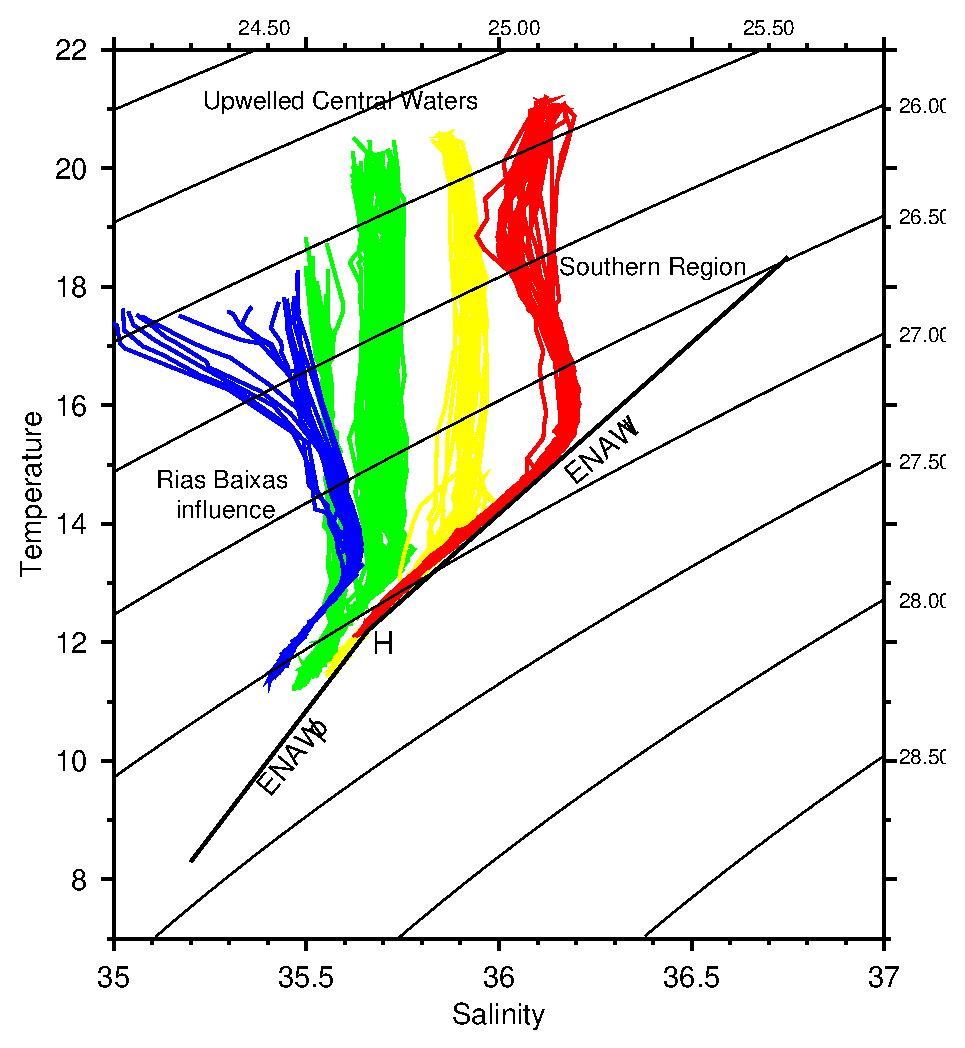
\includegraphics[height=8cm]{ts_diag1}}
  \subfigure[]{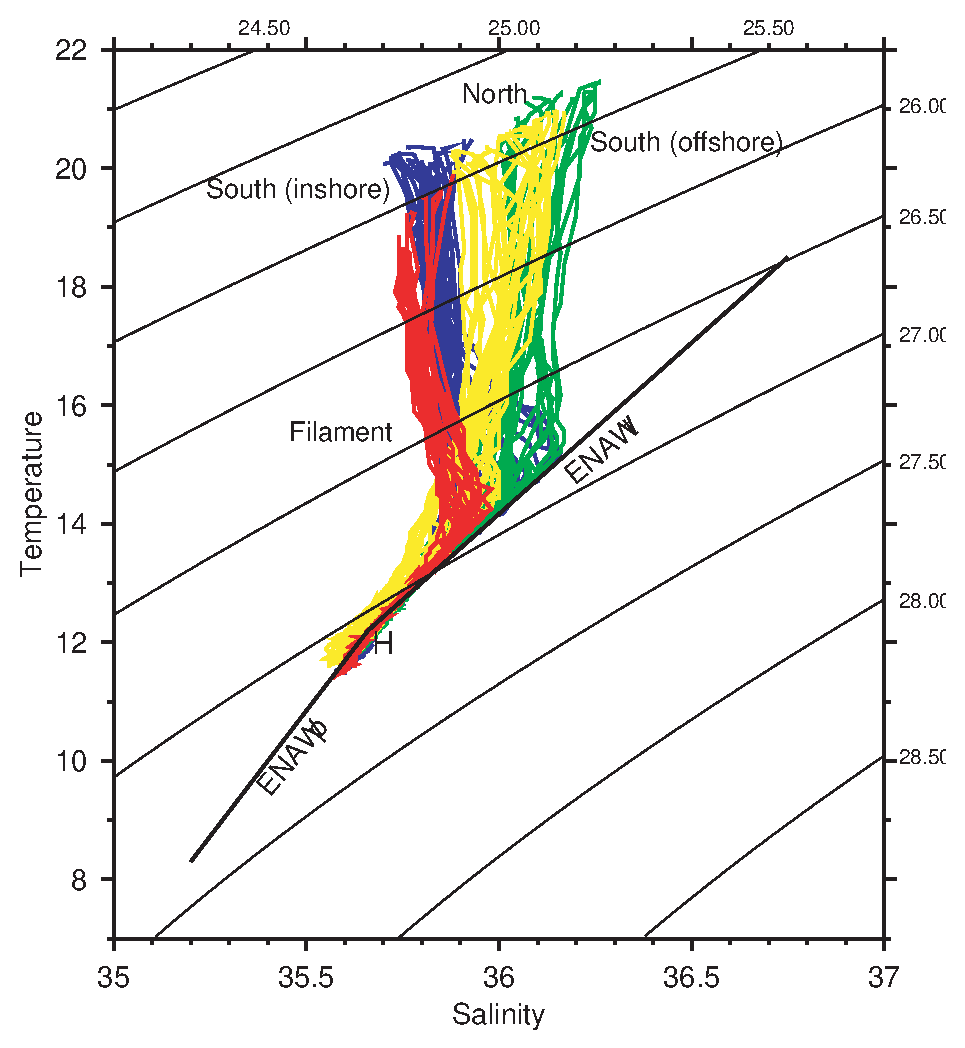
\includegraphics[height=8cm]{ts_diag2}}
   \caption{T/S curves for selected groups of SeaSoar profiles
   between Rias Baixas and southern Portugal revealing the wide
   range of variation alongshore. (a) Characteristic T/S profiles
   of the different upper-layer sub-ambiences likely to be found
   in the Iberian Atlantic coast, (b) strong contrast of the Cape
   Roca filament with respect to surrounding waters. Also shown
   are the characteristic lines of  \enawp and \enawt [{\it Barton
   et al.,} 2002, in preparation].}
  \label{fig:litts}
\end{figure}

The MIW occupies most of the intermediate layer in the Portuguese
coast (Fig.~\ref{fig:ctdmixing}) and is defined by two cores. The
upper core (800m) is characterized by a relative temperature
maximum, 13\deg C, and salinity of 36.4psu,
\citep{Ambar79,Fiuza97} concentrated against the slope in close
relation with the poleward PSU. The MIW lower core (at 1200m) is
better characterized by its salinity maximum, 36.6psu and
temperature of 12.2\deg C \citep{Ambar79}. The lower core is
generally broader and more variable, but on the mid-slope is
strong and persistent \citep{Hamann96}. The MIW is modified along
the Portuguese coast by mixing with the overlying \enaw and so
loses its original characteristics as it progresses northwards
(becoming colder and less saline) until it reaches Cape Finisterre
(43\deg N). There \citet{Rios92} found a strong salinity front,
beyond which the MIW presence was significantly decreased.

In the bottom layer, below 1300m, an isopycnic layer of low
temperature and salinity is commonly found as a result of strong
mixing between the MIW and North Atlantic Deep Water (NADW) on its
way to the south \citep{Ambar94}.

\section{Eastern Boundary Dynamics}\label{sec:upw_theory} Wind-driven
currents are a common feature of the continental shelves and
together with tides they constitute the most energetic,
best-observed and best-modelled form of variability over the
continental margins \citep{Brink98}. In Eastern boundaries,
equatorward winds induce net offshore surface Ekman transport
which brings about transport divergence near the coast and
upwelling of subsurface waters to maintain continuity in the
cross-shelf section. The basic mechanisms of wind-driven coastal
upwelling are well understood and there are several excellent
reviews of upwelling systems \citep[e.g.][]{Allen80,Brink98}.
Other features associated with forcing of finite extent [e.g.
opposing undercurrent and propagation of upwelling by coastal
trapped waves) were reviewed by \citet{Huthnance81} or
\citet{Brink91}. The Californian upwelling system has been the
subject of the most comprehensive and extensive studies such as
CalCOFI, California Cooperative Fisheries Investigations
\citep{Lynn87}, CODE, Coastal Ocean Dynamics Experiment
\citep[e.g.][]{Kosro86}, OPUS, Organization of Persistent
Upwelling Structures, \citep[e.g.][]{Atkinson86} and CTZ, Coastal
Transition Zone \citep{Strub91}, while other Eastern Boundaries
Systems have raised less international attention, e.g. Peru
\citep{Smith81}, NW Africa \citep{Mittelstaed83}, Benguela
Upwelling System \citep{Andrews80} and  West Iberian Peninsula
with the MORENA, Multidisciplinary Oceanographic Research in the
Eastern boundary of the North Atlantic \citep{Fiuza96} and the
recently concluded OMEX II, Ocean Margin Exchanges
\citep{Huthnance02}.

\subsection{Surface Ekman layer}

Currents varying on time-scales of days or longer tend to be
constrained by geostrophy to flow along depth contours. However,
frictional Ekman layers together with local, non-linear and time
dependent flows may relax the geostrophic constraint and
contribute to the ageostrophy of the flow.

The actual contact between wind forcing and the ocean occurs
within the turbulent surface boundary layer, generally called the
Ekman layer. The depth of this layer, typically 10-100m, is
determined by competition between the stabilising effect of
surface heating and the destabilising effects of turbulence
generation by wind input, but also from surface cooling, breaking
waves, or unstable shears in the water column \citep{Brink98}.

Within the surface boundary Ekman layer, the solution to the
governing equations of motion can be found to be a function of the
vertical coordinate only (see \citealp{Pedlosky87} for a full
description of the equations of motion):
\begin{equation}\label{eq:coord}
  u=u(z); v=v(z); w=w(z)
\end{equation}
so that from the continuity equation
\begin{equation}\label{eq:continuity}
  \frac{\partial u}{\partial x}+\frac{\partial v}{\partial y}
  +\frac{\partial w}{\partial z}=0
\end{equation}

we obtained that $\frac{\partial w}{\partial z}=0$. From the
surface boundary condition of $w(0)=0$, it follows that $w$ must
be zero at all depths. The coordinate system adopted is that in
which $x$ is the cross-shelf coordinate (positive onshore), $y$ is
the alongshore coordinate (positive poleward), and $z$ is the
vertical coordinate (positive upward).

Since the fluid is homogeneous, from the hydrostatic approximation
it follows that the horizontal pressure gradient must be
independent of z, and it is therefore entirely determined by any
geostrophic velocity far from the boundary. Ignoring any flows
associated with horizontal pressure gradients is reasonable as
long as the pressure related flow is not too strong; that is, the
(interior) Rossby number
\begin{equation}\label{eq:rossby}
  R_{o}=\frac{v^{*}}{fL}
\end{equation}
(where $v^{*}$ is a typical interior velocity, $f$ is the Coriolis
parameter and $L$ a representative horizontal length scale) is
small.

The basic force balance is then reduced to the local acceleration,
Coriolis and the vertical gradient of turbulent stress. If the
turbulent stress vanishes at some depth below the mixed layer,
then the equations of motion can be vertically integrated to
describe the Ekman transport ($U_{E}$,$V_{E}$):
\begin{equation}\label{eq:ekmanu}
  \frac{\partial U_{E}}{\partial
  t}-fV_{E}=\frac{1}{\rho}\tau_{0}^{x}
\end{equation}
\begin{equation}\label{eq:ekmanv}
  \frac{\partial V_{E}}{\partial
  t}-fU_{E}=\frac{1}{\rho}\tau_{0}^{y}
\end{equation}

where $U_{E}$,$V_{E}$ are the vertically averaged velocities in
the Ekman layer,$\rho$ is the density in the mixed layer and
$\tau_{0}^{x},\tau_{0}^{y}$  are the wind stress applied at the
surface in the $x$ and $y$ directions. Assuming a wind stress of
the form
\begin{equation}\label{eq:windstress}
  \tau_{0}^{y}=T\cos \omega t
\end{equation}

with no component in the across-shelf $(x)$ direction yields a
solution
\begin{equation}\label{eq:ekmansolu}
  U_{E}=\frac{fT}{\rho}(f^{2}-\omega ^{2})^{-1}\cos \omega t
\end{equation}
\begin{equation}\label{eq:ekmansolv}
  V_{E}=\frac{-\omega T}{\rho}(f^{2}-\omega ^{2})^{-1}\sin \omega t
\end{equation}

where $T$ and $\omega$  are the amplitude and frequency of the
wind stress. In the low frequency limit ($f\gg \omega $),
rotational effects dominate and the Ekman transport is
perpendicular to the wind stress. In the high frequency limit
($f\ll \omega$ ), the transport is downwind but lags by a quarter
cycle.
\begin{figure}
  \centering
  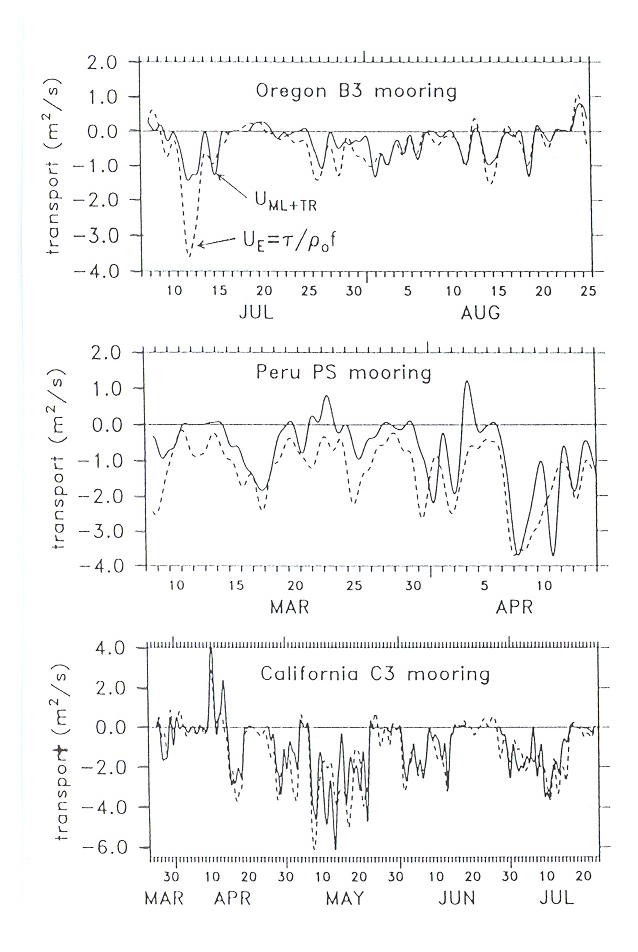
\includegraphics[height=9cm]{fig14new}
  \caption{Time series of cross-shelf transport in the surface
  boundary layer $U(ML+TL)$ (Mixed + Transitional Layer, solid line)
  and the Ekman transport $U_E=\frac{\tau}{(\rho f)}$ (dashed line) from three locations
  during the upwelling season of 1982 [{\it Lentz} 1992].}
  \label{fig:ekmanlayer}
\end{figure}

\begin{figure}
  \centering
  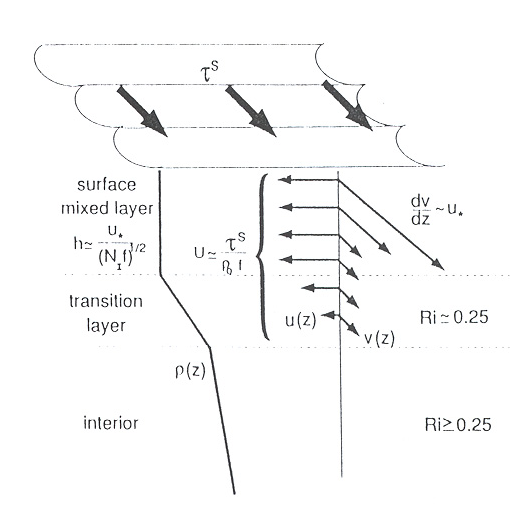
\includegraphics[height=9cm]{fig15new}
  \caption{Schematic summarizing some of the characteristics of
  the surface boundary layer in a coastal upwelling region:
  $u^*=(\frac{\tau^{s}}{\rho_0})^{\frac{1}{2}}$ is the shear
  velocity and $U$ is the cross-shelf transport in the surface
  mixed layer plus the transition layer [{\it Lentz} 1992].}
  \label{fig:upperlayerdiag}
\end{figure}
In most cases, the low frequency limit is an adequate description
which basically reduces eq.~\ref{eq:ekmansolu},~\ref{eq:ekmansolv}
to the theoretical Ekman transport $(\rho f)^{-1}\tau_{0}^{y}$,
which is completely determined in terms of the local value of the
$y$-component of the wind stress. Substantial effort has been
directed towards the verification of the theoretical Ekman
transport \citep{Smith81,Brink83}, especially in coastal upwelling
regions. \citet{Lentz92} reported experiments in 4 coastal
upwelling regions which demonstrated good agreement in magnitude
and variability between the observed cross-shelf Ekman transport
and the theoretical value (Fig.~\ref{fig:ekmanlayer}) but only
when he allowed for the surface Ekman layer being about 25-50\%
deeper than the surface mixed layer including a transitional
stratified layer of near critical Richardson number ($\sim$0.25).
The subtidal surface mixed layer depth was found to be well
described in terms of the wind-induced shear velocity
($u_*=(\frac{\tau_0^y}{\rho_0})$) , the Coriolis parameter ($f$)
and the buoyancy frequency below the mixed layer ($N_I$) in the
form
\begin{equation}\label{eq:ekmandepth}
  \delta _E=\frac{u_*}{(N_If)^{\frac{1}{2}}}
\end{equation}

It was found no account need be made for the surface heat flux and
heat advection as they tend to balance each other in the coastal
upwelling regions studied. Fig.~\ref{fig:upperlayerdiag} shows an
schematic of the upper water column geometry in coastal upwelling
systems.

Secondary pressure related flows can become important and
influence Ekman layer processes. Vorticity of the background flow
allows convergences and divergences in the Ekman transport even
under the effects of a uniform wind \citep{Niiler69}.
\subsubsection{Coastal wind-driven upwelling}
In a coastal context, wind-driven flows can be described by
depth-integrated equations of motion where nonlinearities and
density variations are not allowed:
\begin{equation}\label{eq:winddriven1}
  \frac{\partial U}{\partial t}-fV=-\frac{1}{\rho}h\frac{\partial
  p}{\partial x}+\frac{1}{\rho}(\tau_0^x-\tau_B^x)
\end{equation}
\begin{equation}\label{eq:winddriven2}
   \frac{\partial V}{\partial t}-fU=-\frac{1}{\rho}h\frac{\partial
  p}{\partial y}+\frac{1}{\rho}(\tau_0^y-\tau_B^y)
\end{equation}
\begin{equation}\label{eq:winddriven3}
\frac{\partial U}{\partial x}+\frac{\partial V}{\partial y}=0
\end{equation}

where $U,V$ are the cross-shore and along-shore depth-integrated
transports, $h(x)$ is the water depth and p is the pressure. A
rigid lid is assumed for the surface boundary because interest is
confined to relatively short spatial scales compared to the
barotropic radius of deformation (natural horizontal scale for
upwelling and expected distance from the coast of the upwelling
front). The bottom stress will be assumed to be proportional to
the depth-averaged current,
\begin{equation}\label{eq:botstress1}
\tau_B^x=\rho rh^{-1}U
\end{equation}
\begin{equation}\label{eq:botstress2}
\tau_B^y=\rho rh^{-1}V
\end{equation}

where $r$ is the drag coefficient.

Solving eq.~\ref{eq:winddriven1},~\ref{eq:winddriven2} and
~\ref{eq:winddriven3} is easier if the long-wave approximation is
made. This assumes that alongshore scales are large relative to
cross-shelf scales, ($Ly \gg Lx$) , time scales of interest are
long relative to the inertial period, ($f \gg \omega$)(more
specifically, longer than the sum of the inertial period and the
frictional e-folding time dependent on the depth \citep{Dalu90})
and finally that frictional effects are not too large ($f\gg
rh^{-1}$). This approximation is justifiable as the major
upwelling systems are induced by large scale wind patterns
characterised by alongshore spatial scales larger than the
shelf-slope width and weather changes do occur at time scales
longer than  several days.

\begin{figure}
  \centering
  \includegraphics[height=9cm]{fig16a}
  \includegraphics[height=9cm]{fig16b}
  \caption{Aircraft wind measurements acquired during CODE 2
  experiment (summer 1982) from which (1) wind stress (Pa) and (2)
  wind stress curl (Pa/100km) were computed. (3) and (4) show
  simulations from a simple, two layer, vertically integrated
  model of coastal upwelling. They represent the upper-layer
  thickness (in m) after 24 hours of simulation using observed
  wind stresses, (3) without curl and (4) with curl. Note how the
  nonzero stress curl enhanced coastal upwelling, the greatest
  effects being around the areas of largest observed curl values
  [{\it Enriquez and Friehe}, 1995].}
  \label{fig:capewind}
\end{figure}


The long-wave approximation has as a main consequence that
alongshore flows are stronger than cross-shelf flows which is a
common characteristic of upwelling systems
\citep[e.g.][]{Batteen97}, and that the alongshore flow is in
geostrophic balance due to the scaling of eq.~\ref{eq:winddriven1}
(cross-shelf wind and bottom stress and local cross-shelf
acceleration can be neglected relative to the Coriolis and
pressure terms):
\begin{equation}\label{eq:geost}
  -fV=-\frac{1h}{\rho}\frac{\partial p}{\partial x}
\end{equation}
The main failure of the scaling approximation resides in the
alongshore uniformity of the wind and topography. It is well
established that coastal irregularities such as capes or bays may
induce wind stress variations (Fig.~\ref{fig:capewind}) which are
of major importance in the evolution and final equilibrium state
of upwelling systems \citep[e.g.][]{Haynes93,Enriquez95}.
Furthermore, lateral wind stress gradients can induce Ekman
pumping and enhance the baroclinicity of the alongshore flow
\citep{Brink87,Batteen92}.

Nevertheless the above simplified model can be solved for a
spatially uniform constant alongshore wind $\tau_0^y=T$, with no
alongshore variations allowed,$\frac{\partial}{\partial y}=0$ so
that continuity reduces to
\begin{equation}\label{eq:consimp}
 \frac{\partial U}{\partial x}=0
\end{equation}
On the coastal boundary the no cross-shelf flow must applied so
that the depth-integrated cross-shelf transport must vanish
everywhere, which reduces eq.~\ref{eq:winddriven2} to
\begin{eqnarray}\label{eq:depthmotion}
 &U=-\frac{1}{f}\frac{\partial V}{\partial t}+
 \frac{1}{\rho f}\tau_0^y-\frac{rV}{fh}=0  \\
 & \equiv U_I+U_{E0}+U_{EB}=0 \nonumber
\end{eqnarray}
where $U_I$ is the interior transport, $U_{E0}$ is the surface
Ekman transport and $U_{EB}$ is the bottom Ekman transport.
Basically, the surface Ekman flow is compensated by flows deeper
in the water column sufficiently far from the coastal boundary
where lateral friction and vertical velocities can not be
neglected. Solving eq.~\ref{eq:depthmotion} for $V$ is
straightforward in a system starting from the rest, i.e. $V=0$ at
$t=0$:
\begin{equation}\label{eq:depthsol1}
  V=\frac{hT}{r\rho}[1-\exp(-rh^{-1}t)]
\end{equation}
\begin{figure}
  \centering
  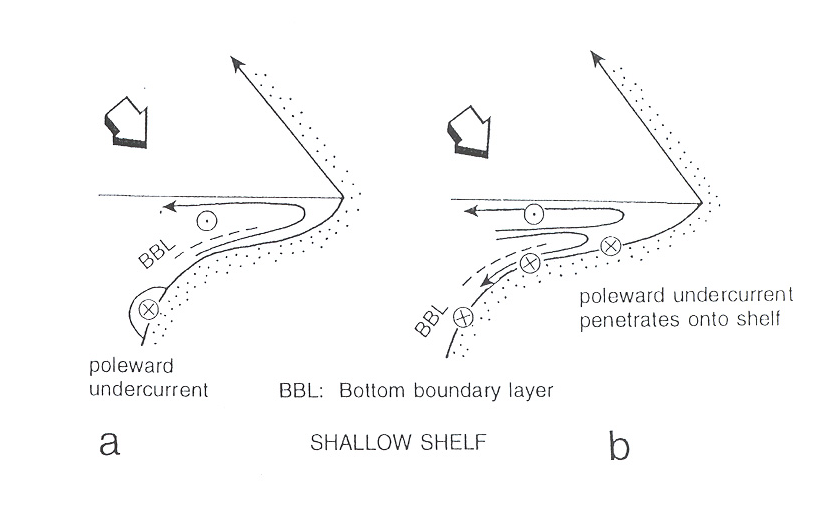
\includegraphics[height=8cm]{fig18new}
  \caption{Schematic of coastal upwelling: (a) upwelling over a
  shallow frictional shelf where the equatorward flow on the shelf
  penetrates to the bottom and bottom Ekman transport is onshore,
  supplying the upwelling waters; (b) upwelling over a shallow
  frictional shelf when the poleward undercurrent penetrates the
  shelf and the bottom Ekman layer transport is offshore and
  upwelling water are supplied from middepth
  [{\it Hill et al.,}, 1998].}
  \label{fig:polewdiag}
\end{figure}

It can be seen that for $t \ll rh^{-1}$ the alongshore flow
accelerates steadily at a rate,
\begin{equation}\label{eq:depthsol2}
  V\approx \frac{T}{\rho}t
\end{equation}
so that the surface Ekman flow is compensated mainly from the
interior flow. At larger times, $t \gg rh^{-1}$, the interior flow
disappears $(\frac{\partial V}{\partial t}=0)$ reaching a steady
state and the surface Ekman flow is now compensated entirely by
the bottom Ekman flow, i.e. the flow is entirely frictional
determined (Fig.~\ref{fig:polewdiag}). More generally, however,
this equilibrium is not reached; acceleration, stratification and
the ignored along-shore pressure gradients also distribute the
stress and upwelling through the water column \citep{Huthnance95}.

Upwelling systems are generally highly time-dependent and respond
rapidly to wind stress fluctuations. Initially the upwelling
favourable winds drive an offshore Ekman flow which forces the
interface (seasonal thermocline) beneath the upper layer to rise
near the coast at a distance defined by the Rossby radius of
deformation,$R'=\frac{HN}{f}$ where $H$ is the depth of the mixed
surface layer, usually taken to be the same as the surface Ekman
layer, and $N$ is the buoyancy frequency below the mixed layer,
generating geostrophically balanced alongshore currents, namely an
equatorward coastal jet and a poleward undercurrent. The upwelled
water band width,$R'$, will be also governed by the time
integrated offshore Ekman transport , so that the band tends to be
narrower where the upwelling-favorable winds are intermittent
(e.g. Oregon) and broader where winds are steadier and stronger
(e.g. California) \citep{Szoeke84}. Sufficiently far
$(>\frac{HN}{f})$ from the coast the inflow is uniform through
depth without a vertical component, as described by
eq.~\ref{eq:depthmotion}. In the presence of stratification, an
upper layer of characteristics $H_1N_1$ over a $2^{nd}$ layer of
$H_2N_2 (H_1N_1 > H_2N_2)$ gives a majority of upwelling inflow in
the upper layer within $(>\frac{H_1N_1}{f})$ of the coast. The
magnitude of the alongshore current in the coastal jet and the
horizontal scale of the coastal jet also depend on stratification
increasing as $N^2$ increases, whereas weaker stratification
enables the front to develop faster \citep{Allen95}.

The time evolution of the system will also be affected by
diffusive processes induced by upwelling and mixing, which reduce
the coastal layer depth and density stratification  $(H_1N_1)$ and
hence the offshore scale \citep{Szoeke84}. One non-linear aspect
of the system is that the front and surface jet are advected
offshore by Ekman drift although they will be generally limited to
the shelf, stopping at any shelf break \citep{Huthnance95}. The
absence of a front over the shelf has been related to sustained
favourable upwelling winds, for example in Peru (15\deg S) or off
central California \citep{Smith81,Brink83}.
\begin{figure}
  \centering
  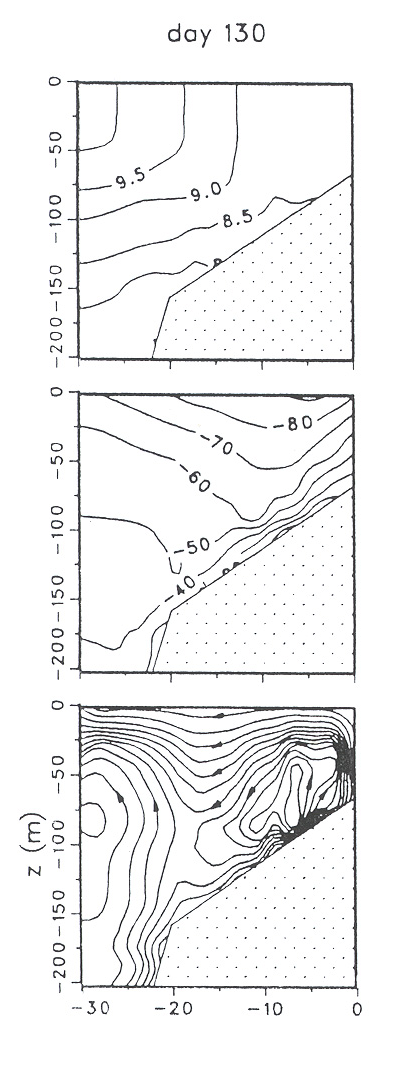
\includegraphics[height=12cm]{fig17new}
  \caption{Prediction from a combined two-dimensional circulation
  model and one dimensional mixed-layer model of cross-shelf
  structures of Temperature ($C$)(top), alongshore velocity
  (\velc)(middle), and stream function (\mixc)(bottom). On day 130
  the equatorward wind stress is the strongest and the upwelling
  front moves to the outer shelf. Upwelling takes place in two
  narrow areas, one at the coast and the other on the seaward side
  of the front. In association with the convergence and divergence
  of the upper layer transport, a prominent double-cell
  circulation is formed
  [{\it Chen and Wang,}, 1990].}
  \label{fig:cellcirc}
\end{figure}

The front itself is characterised by relatively large horizontal
density and alongshore velocity $(v)$ gradient near surface and
large vertical gradients in $v$ at mid-depth. There is
occasionally a convergence of near-surface offshore flow at the
front that results in a general increase in depth of the surface
turbulent boundary layer across the front \citep{Allen95} and that
has been suggested to constitute a two cell pattern
(Fig.~\ref{fig:cellcirc}) \citep{Chen90}. In response to strong
winds the front would display a tendency for the surface isotherms
to parallel the bottom topography as a result of advection by a
nearly uniform Ekman transport while weaker winds produce a
complex contouring front \citep{Brink83}.

A large variety of studies acknowledges the important role of
shelf/slope topography in upwelling, a factor which has been
neglected to this point in the review. Complex coastal features
such as capes, ridges, submarine canyons and submarine banks,
which have along-shelf scales that are comparable to or smaller
than cross-shelf scales produce flow structures that differ
fundamentally from those addressed by the classical theory and are
often the site of significant cross-isobath flows
\citep{Trowbridge98}.

The classical assumption of an along-shelf length scale much
larger than the cross-shelf length scale leads to an along-shelf
flow which is nearly geostrophic even when the Rossby $(R_0)$ and
vertical Ekman numbers ($E_v=\frac{A_v}{fH^2}$  where $A_v$ is the
vertical mixing coefficient assumed independent of $z$, and $H$ is
a typical vertical scale ) approach unity as shown by the scaling
of the momentum equations \citep{Trowbridge98}. The geostrophic
balance is only slightly altered by changes in the cross-shelf
velocity caused by ageostrophic processes (mixing and local
acceleration). On the other hand, the cross-shelf velocity is
likely to be ageostrophic even when the Rossby and Ekman numbers
are small, so that small changes in the along-shelf velocity have
a major impact on the cross-shelf flow.

Another source of time dependence in upwelling systems is brought
about by propagation of disturbances from remote locations by
coastally trapped waves (see later) which induce variability on
time scales of from 3 to 10 days \citep{Denbo87}.
Fig.~\ref{fig:3dupwdiag} shows an schematic of the common features
that can be expected in a coastal upwelling system.
\begin{figure}
  \centering
  \includegraphics[height=13cm]{upwfig}
  \caption{Schematic of an upwelling system showing the varied
  range of possible physical processes and the complex 3
  dimensionality of the system
  [{\it Hill et al.,}, 1998].}
  \label{fig:3dupwdiag}
\end{figure}

Most coastal upwelling is produced by along-shelf wind stresses
and may be altered greatly by short along-shelf scales in the
coastline \citep{Crepon82,Crepon84,Haynes93,Wang97} in turn
altering the local direction of the wind relative to the coastline
and reducing or enhancing upwelling/downwelling locally.
Consequently, along-shelf variations in the pressure gradient will
be introduced, which may then propagate along the coast as CTW's
\citep{Crepon82} and give rise to a countercurrent below the
thermocline opposing the prevailing winds \citep{Suginohara82}.

\citet{Enriquez95} showed that the wind small-scale spatial
variability near Pt. Arena (California) had characteristic scales
much smaller than the scales of synoptic atmospheric pressure
patterns and calculated local wind stress curl five times larger
than those obtained from long-term ship data using bulk
aerodynamic formulas. The local coastline (cape) was responsible
for a sustained curl pattern which modified the dynamical response
of the coastal water to the applied wind stress and resulted in
local enhancement of upwelling downwind of the cape during
favourable winds (Fig.~\ref{fig:capewind}). The theoretical study
of \citet{Crepon84} also supports upwelling enhancement downwind
of a cape relating the intensity to the offshore scale of the cape
while the geometry of the cape does not change the process
qualitatively. The cape, like the alongshore variability in the
wind-stress, generates an undercurrent in the opposite direction
to the wind.

The shelf geometry itself also influences the upwelling system.
Shallow wide shelves without poleward undercurrent generate large
bottom friction and larger Ekman onshore transport which in turn
limits the acceleration of the jet so weaker surface jets are
expected. The front is wider and occurs further offshore
\citep{Allen95}. The concentration of depth contours tends to
guide and strengthen currents along the continental slope where
the sea floor slope exerts an stabilising effect
\citep{Huthnance81}. In those steep shelves, the vertical
gradients of v tend to be more geostrophically balanced so that
the frictional bottom boundary layer is weaker and carries less
fraction of onshore flow. Near-surface density gradients tend to
occur near the coast so that offshore-displaced upwelling fronts
may not be observed. \citep{Allen95}.

\subsection{Instabilities}

Mathematical models investigating the dynamics of upwelling,
filaments, squirts and eddies suggest that the phenomena result
from instability of alongshore currents, and they all point toward
baroclinic instability as being an important process. Several of
this models also developed small-scale disturbances along fronts
and indicated that other instability mechanisms are involved in
their generation as well \citep{McCreary91}. In those mathematical
models, meanders and eddies increased in scale as the system
adjusted toward equilibrium, apparently for different dynamical
reasons in each case.

\citet{McCreary91} reviewed previous stability models and
experimented with simpler models to infer two types of
instability, as also found by \citet{Barth94} with continuous
forms of stratification and coastal current. These two
instabilities are: shorter-scale frontal instability depending on
gradients of sea-surface temperature, trapped to the front and
upper column and extracting potential energy; a larger-scale
``traditional'' baroclinic instability manifested later in
filament development. The vertical shear between an equatorward
upwelling front jet and the poleward undercurrent give a mechanism
for the generation of baroclinic instabilities as shown by model
experiments in the Californian shelf by \citet{Batteen89}.

\subsection{Coastal trapped waves}
The sudden change in bathymetry at the shelf-edge imply a large
potential vorticity gradient and provide conditions that lead to
the trapping of certain wave motions called continental shelf
waves or coastal trapped waves \citep{Huthnance81}. These waves
are commonly generated by transient winds \citep{Adams69} and
propagate along the shelf-edge, cyclonically around the ocean at
sub-inertial frequencies \citep{Huthnance86}. They arise from the
conservation of potential vorticity as water passes over uneven
bottom topography:
\begin{equation}\label{eq:ctw}
  \frac{d(\frac{f+\xi}{h})}{dt}=0
\end{equation}

According to eq.~\ref{eq:ctw}, if a fluid column is displaced up
or down a slope, vortex stretching or compression will tend to
move the water back to where it was originally. This results in
long, sub-inertial wave forms which propagate cyclonically in the
northern hemisphere, with the shallow water on their right. They
tend to decay off-shelf but some may be at their most energetic
over the slope \citep{Huthnance95}.

A numerical investigation by \citet{Suginohara74,Suginohara82} of
a coastal ocean with cross-shelf topography and vertical
stratification underlies the importance of coastal trapped waves
in the development of an upwelling circulation including that of a
poleward flow of about 2\velc. \citet{Denbo87} and others, have
shown the importance of Coastal trapped waves in wind-driven
currents in the CODE area.

\subsection{Poleward slope flow}
Current along the continental slope can and do occur with non-zero
time-average and velocities exceeding or opposing those to either
side of the adjacent shelf and ocean \citep{Huthnance95}. Poleward
slope currents are in fact widespread in Eastern boundaries, and
often flow against prevailing equatorward winds as in seasonal
upwelling systems (e.g. California) , which suggests a
large-scale, non-local forcing of the current. The precise
cross-shelf distribution of the flow depends upon the character of
the forcing balanced by alongshore pressure gradient, friction and
acceleration.

The steep topography of the slope and the influence of Earth's
rotation are the primary factors aligning barotropic currents
along the depth contours and both continuity arguments and
potential vorticity conservation can explain the anchorage of the
slope current along the slope region. Usually the poleward flow is
located at the shelf break or over the continental slope with a
width of the order of 20-100km and current speeds of order of
10\velc.

The several potential forcing forces are:
\begin{itemize}
  \item Freshwater runoff resulting in a baroclinic coastal current
\citep{Hill98} which can include the shelf edge for sufficient
runoff and narrow shelf.
  \item Alongshore pressure gradients imposed by the ocean and
incorporating density forcing combined with the slope bathymetry
to drive the slope poleward current.
\end{itemize}

The latter one is of most general ubiquity and was described by
\citet{Huthnance84}. It was termed JEBAR, Joint Effect of
Baroclinicity And Relief, and refers to the dynamical adjustment
of the density-induced pressure gradient to the bottom slope when
the zonally orientated density surfaces intersects a meridional
sloping boundary (Fig.~\ref{fig:jebar}). Under no net cross-shore
transport and assuming the same meridional density gradient is
affecting both the shelf and the ocean, the alongshore sea-level
slope is proportional to the bottom depth. On the shelf the
sea-level drop is less than in the ocean then generating an
offshore pressure gradient which drives the poleward flow along
the slope. This pressure gradient increases along-slope therefore
accelerating the flow until friction becomes important and a
steady state is reached.
\begin{figure}
  \centering
  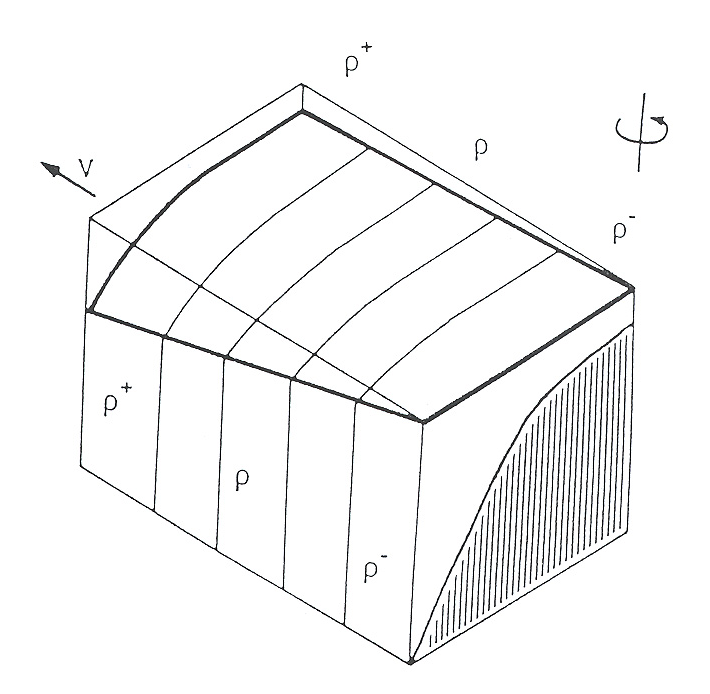
\includegraphics[height=8cm]{fig20new}
  \caption{A simple JEBAR model. The sea surface over a
  shelf-slope region is shown as a thick line. Density increases
  alongshore and continuity is maintained by a condition of no net
  cross-slope transport. Sea level declines more gently over
  shallow water than over deep water hence a steepening
  cross-slope sea level difference develops which drives a
  strengthening along-slope current
  [{\it Hill,}, 1998].}
  \label{fig:jebar}
\end{figure}


In upwelling systems, there also exist local terms forcing the
poleward undercurrent which are highly influenced by alongshore
variability \citep{Hill98}. Some of these possible forcings for
undercurrent poleward flow in the face of equatorward wind stress
are: remote forcing, relaxation of equatorward wind, the positive
curl of equatorward wind stress or thermohaline forcing
\citep{McCreary87}. Along-slope variations in topography could
allow the necessary alongshore pressure gradient to drive the
undercurrent as alongshore variations in the wind stress field
would do too \citep{Hill98}. There are multiple observational
evidences of the poleward undercurrent in the Oregon upwelling
system but only scattered ones in the Eastern Atlantic coast like
N.West Africa where the poleward undercurrent flows below the
shelf break \citep{Mittelstaed75,Barton90} and on the Portuguese
slope where six month long measurements of poleward flow were
recorded by \citet{Ambar84,Ambar85} at levels below 200m in bottom
depth less than 1000m. Off Oregon the shelf break is less sharp
and so the undercurrent is partly on the shelf \citep{Huyer76}.
